%<dscrpt>Fichier de déclarations Latex à inclure au début d'un élément de cours.</dscrpt>

\documentclass[a4paper]{article}
\usepackage[hmargin={1.8cm,1.8cm},vmargin={2.4cm,2.4cm},headheight=13.1pt]{geometry}

%includeheadfoot,scale=1.1,centering,hoffset=-0.5cm,
\usepackage[pdftex]{graphicx,color}
\usepackage[french]{babel}
%\selectlanguage{french}
\addto\captionsfrench{
  \def\contentsname{Plan}
}
\usepackage{fancyhdr}
\usepackage{floatflt}
\usepackage{amsmath}
\usepackage{amssymb}
\usepackage{amsthm}
\usepackage{stmaryrd}
%\usepackage{ucs}
\usepackage[utf8]{inputenc}
%\usepackage[latin1]{inputenc}
\usepackage[T1]{fontenc}


\usepackage{titletoc}
%\contentsmargin{2.55em}
\dottedcontents{section}[2.5em]{}{1.8em}{1pc}
\dottedcontents{subsection}[3.5em]{}{1.2em}{1pc}
\dottedcontents{subsubsection}[5em]{}{1em}{1pc}

\usepackage[pdftex,colorlinks={true},urlcolor={blue},pdfauthor={remy Nicolai},bookmarks={true}]{hyperref}
\usepackage{makeidx}

\usepackage{multicol}
\usepackage{multirow}
\usepackage{wrapfig}
\usepackage{array}
\usepackage{subfig}


%\usepackage{tikz}
%\usetikzlibrary{calc, shapes, backgrounds}
%pour la présentation du pseudo-code
% !!!!!!!!!!!!!!      le package n'est pas présent sur le serveur sous fedora 16 !!!!!!!!!!!!!!!!!!!!!!!!
%\usepackage[french,ruled,vlined]{algorithm2e}

%pr{\'e}sentation du compteur de niveau 2 dans les listes
\makeatletter
\renewcommand{\labelenumii}{\theenumii.}
\renewcommand{\thesection}{\Roman{section}.}
\renewcommand{\thesubsection}{\arabic{subsection}.}
\renewcommand{\thesubsubsection}{\arabic{subsubsection}.}
\makeatother


%dimension des pages, en-t{\^e}te et bas de page
%\pdfpagewidth=20cm
%\pdfpageheight=14cm
%   \setlength{\oddsidemargin}{-2cm}
%   \setlength{\voffset}{-1.5cm}
%   \setlength{\textheight}{12cm}
%   \setlength{\textwidth}{25.2cm}
   \columnsep=1cm
   \columnseprule=0.5pt

%En tete et pied de page
\pagestyle{fancy}
\lhead{MPSI-\'Eléments de cours}
\rhead{\today}
%\rhead{25/11/05}
\lfoot{\tiny{Cette création est mise à disposition selon le Contrat\\ Paternité-Pas d'utilisations commerciale-Partage des Conditions Initiales à l'Identique 2.0 France\\ disponible en ligne http://creativecommons.org/licenses/by-nc-sa/2.0/fr/
} }
\rfoot{\tiny{Rémy Nicolai \jobname}}


\newcommand{\baseurl}{http://back.maquisdoc.net/data/cours\_nicolair/}
\newcommand{\urlexo}{http://back.maquisdoc.net/data/exos_nicolair/}
\newcommand{\urlcours}{https://maquisdoc-math.fra1.digitaloceanspaces.com/}

\newcommand{\N}{\mathbb{N}}
\newcommand{\Z}{\mathbb{Z}}
\newcommand{\C}{\mathbb{C}}
\newcommand{\R}{\mathbb{R}}
\newcommand{\D}{\mathbb{D}}
\newcommand{\K}{\mathbf{K}}
\newcommand{\Q}{\mathbb{Q}}
\newcommand{\F}{\mathbf{F}}
\newcommand{\U}{\mathbb{U}}
\newcommand{\p}{\mathbb{P}}


\newcommand{\card}{\mathop{\mathrm{Card}}}
\newcommand{\Id}{\mathop{\mathrm{Id}}}
\newcommand{\Ker}{\mathop{\mathrm{Ker}}}
\newcommand{\Vect}{\mathop{\mathrm{Vect}}}
\newcommand{\cotg}{\mathop{\mathrm{cotan}}}
\newcommand{\sh}{\mathop{\mathrm{sh}}}
\newcommand{\ch}{\mathop{\mathrm{ch}}}
\newcommand{\argsh}{\mathop{\mathrm{argsh}}}
\newcommand{\argch}{\mathop{\mathrm{argch}}}
\newcommand{\tr}{\mathop{\mathrm{tr}}}
\newcommand{\rg}{\mathop{\mathrm{rg}}}
\newcommand{\rang}{\mathop{\mathrm{rg}}}
\newcommand{\Mat}{\mathop{\mathrm{Mat}}}
\newcommand{\MatB}[2]{\mathop{\mathrm{Mat}}_{\mathcal{#1}}\left( #2\right) }
\newcommand{\MatBB}[3]{\mathop{\mathrm{Mat}}_{\mathcal{#1} \mathcal{#2}}\left( #3\right) }
\renewcommand{\Re}{\mathop{\mathrm{Re}}}
\renewcommand{\Im}{\mathop{\mathrm{Im}}}
\renewcommand{\th}{\mathop{\mathrm{th}}}
\newcommand{\repere}{$(O,\overrightarrow{i},\overrightarrow{j},\overrightarrow{k})$}
\newcommand{\cov}{\mathop{\mathrm{Cov}}}

\newcommand{\absolue}[1]{\left| #1 \right|}
\newcommand{\fonc}[5]{#1 : \begin{cases}#2 \rightarrow #3 \\ #4 \mapsto #5 \end{cases}}
\newcommand{\depar}[2]{\dfrac{\partial #1}{\partial #2}}
\newcommand{\norme}[1]{\left\| #1 \right\|}
\newcommand{\se}{\geq}
\newcommand{\ie}{\leq}
\newcommand{\trans}{\mathstrut^t\!}
\newcommand{\val}{\mathop{\mathrm{val}}}
\newcommand{\grad}{\mathop{\overrightarrow{\mathrm{grad}}}}

\newtheorem*{thm}{Théorème}
\newtheorem{thmn}{Théorème}
\newtheorem*{prop}{Proposition}
\newtheorem{propn}{Proposition}
\newtheorem*{pa}{Présentation axiomatique}
\newtheorem*{propdef}{Proposition - Définition}
\newtheorem*{lem}{Lemme}
\newtheorem{lemn}{Lemme}

\theoremstyle{definition}
\newtheorem*{defi}{Définition}
\newtheorem*{nota}{Notation}
\newtheorem*{exple}{Exemple}
\newtheorem*{exples}{Exemples}


\newenvironment{demo}{\renewcommand{\proofname}{Preuve}\begin{proof}}{\end{proof}}
%\renewcommand{\proofname}{Preuve} doit etre après le begin{document} pour fonctionner

\theoremstyle{remark}
\newtheorem*{rem}{Remarque}
\newtheorem*{rems}{Remarques}

\renewcommand{\indexspace}{}
\renewenvironment{theindex}
  {\section*{Index} %\addcontentsline{toc}{section}{\protect\numberline{0.}{Index}}
   \begin{multicols}{2}
    \begin{itemize}}
  {\end{itemize} \end{multicols}}


%pour annuler les commandes beamer
\renewenvironment{frame}{}{}
\newcommand{\frametitle}[1]{}
\newcommand{\framesubtitle}[1]{}

\newcommand{\debutcours}[2]{
  \chead{#1}
  \begin{center}
     \begin{huge}\textbf{#1}\end{huge}
     \begin{Large}\begin{center}Rédaction incomplète. Version #2\end{center}\end{Large}
  \end{center}
  %\section*{Plan et Index}
  %\begin{frame}  commande beamer
  \tableofcontents
  %\end{frame}   commande beamer
  \printindex
}


\makeindex
\begin{document}
\noindent

\debutcours{Sommations}{1.2 \tiny{ le \today}}

\section{Sommer et récolter}
\subsection{Notations}
Les symboles $\sum$ et $\prod$ sont utilisés respectivement pour désigner une somme d'un nombre fini de \emph{termes} \index{termes} ou un produit d'un nombre fini de \emph{facteurs} \index{facteurs}. Autour de ces symboles figure un \emph{nom local} qui permet de désigner le terme ou le facteur. On utilise aussi \emph{variable locale} ou \emph{variable muette} \index{variable locale, variable muette}
\begin{figure}[h]
  \centering
  \subfloat[sur des petits pois dans leur cosse]{
    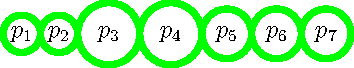
\includegraphics[scale=0.7]{./C2003_2.pdf}
    \label{fig:C2003_1}
  }
  \hspace{1cm}
  \subfloat[sur un ensemble $\mathcal{C}$ de coquillettes]{
    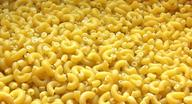
\includegraphics[scale=0.9]{./C2003_3.jpg}
    \label{fig:C2003_3}
  }
  \hspace{1cm}
  \subfloat[sur un ensemble $\mathcal{T}$ de points]{
    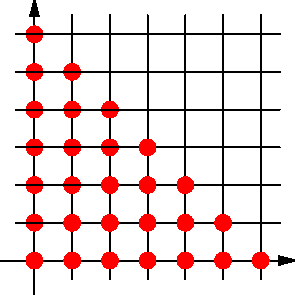
\includegraphics[scale=0.7]{C2003_1.pdf}
    \label{fig: C2003_2}
  }
  \caption{Des sommations ...}
\end{figure}
\begin{itemize}
  \item La masse des petits pois est notée
  \begin{displaymath}
  \sum_{i=1}^7\mu(p_i)  
  \end{displaymath}
  où la lettre $i$ est le nom du nombre permettant de repérer le petit pois (désigné par $p_i$) dans la cosse. La lettre $\mu$ désigne la \emph{fonction} donnant la masse d'un pois. Comme les indices à considérer forment un \emph{intervalle entier} \index{intervalle entier}, on utilise une notation au dessus et au dessous du symbole. Noter l'analogie avec la notation des intégrales.\newline
  On utilise une notation particulière pour les intervalles entiers. Si $a$ et $b$ sont des entiers relatifs avec $a\leq b$:
  \begin{displaymath}
    \llbracket a , b \rrbracket = \left\lbrace a,a+1, \cdots, b\right\rbrace 
  \end{displaymath}

  \item La masse des coquillettes est notée 
  \begin{displaymath}
    M = \sum_{c \in \mathcal{C}}\mu(c)
  \end{displaymath}
  Cette fois $c$ est le nom d'une coquillette de l'ensemble. On peut numéroter les coquillettes une par une de $1$ à $N$ et utiliser un nom de l'indice:
  \begin{displaymath}
    M = \sum_{i=1}^N \mu(c_i)
  \end{displaymath}
  mais cela n'est pas obligatoire, la première notation est aussi commode.
  
  \item Soit $\mathcal T$ l'ensemble des couples d'entiers naturels réprésentés par les points rouges de la figure. Pour tout point $P\in \mathcal T$, on pose $\mu(P)= ij$ si $P=(i,j)$. On considère la somme
\begin{displaymath}
S = \sum_{P\in \mathcal T} \mu(P) = \sum_{(i,j)\in \mathcal T} ij                                                                                                                                                                                         \end{displaymath}
On trouvera une expression pour cette somme à la fin de la section suivante.
\end{itemize}

On peut combiner les notations précédentes:
\begin{displaymath}
  \left( \sum_{i=1}^pa_i\right)\left( \sum_{i=1}^qb_i\right)
=   \left( \sum_{i=1}^pa_i\right)\left( \sum_{j=1}^qb_j\right)
= \sum_{(i,j)\in \llbracket 1,p\rrbracket \times \llbracket 1,q \rrbracket}a_ib_j
\end{displaymath}
Noter que les noms $i$ sont \emph{locaux} à chaque somme, c'est à dire qu'ils n'ont de signification qu'à l'intérieur de la somme qui les définit. Il n'y a donc pas de problème à utiliser la première manière d'écrire. Les problèmes surviendront lorsque l'on développera le produit car les deux noms se trouveront alors dans la même expression. Il faudra trouver des noms différents pour les deux objets.

\subsection{Changement de nom d'indice}
Dans une addition l'ordre des termes est sans importance, on peut donc les permuter et repérer ce nouvel ordre avec un nouvel indice sans changer la valeur de la somme.

Mise en \oe{}uvre pratique.
\begin{itemize}
  \item Former une relation entre l'ancien nom et le nouveau nom. Exprimer l'ancien nom en fonction du nouveau.
  \item Vérifier que lorsque l'ancien nom décrit son intervalle entier de définition, le nouveau nom décrit un intervalle entier et préciser soigneusement cet intervalle et ses bornes.
  \item Remplacer dans la somme les bornes de l'ancien intervalle par les bornes du nouveau et l'ancien nom par son expression en fonction du nouveau.
\end{itemize}

Exemple pour la somme des entiers consécutifs $S=\sum_{k\in \{1,\cdots,n\}}k$. On somme en allant de $n$ à $1$. 
\begin{itemize}
  \item Ancien nom $k$, nouveau nom $i$, relation $i = n+1-k$, on exprime $k=n+1-i$.
  \item Lorsque $k$ décrit $1,\cdots,n$, $i$ décrit $n,\cdots,1$. Les bornes de l'intervalle décrit par $i$ restent $1$ et $n$.
  \item Remplacement :
\begin{displaymath}
 S=\sum_{k\in \{1,\cdots,n\}}k = \sum_{i\in \{1,\cdots,n\}}(n+1-i)
\end{displaymath}
\end{itemize}
Le nom de la variable est sans importance. On en déduit 
\begin{displaymath}
\left. 
\begin{aligned}
  &S  &= \sum_{k\in \{1,\cdots,n\}}(n+1-k)\\
  &S = \sum_{i\in \{1,\cdots,n\}}(n+1-i)&= \sum_{k\in \{1,\cdots,n\}}(n+1-k)
\end{aligned}
\right\rbrace \Rightarrow
2S = \sum _{k\in \{1,\cdots,n\}}(n+1)= n(n+1)\Rightarrow S =\frac{1}{2}n(n+1)
\end{displaymath}
Autre méthode : avec un tableau carré $(n+1)\times(n+1)$.
\begin{center}
\begin{tabular}{|c|c|c|c|c|c|}
\hline
                  &          &          &\phantom{$\times$}&\phantom{$\times$}&\phantom{$\times$} \\ \hline
$\times$          &          &          &                  &                  & \\ \hline
$\times$          & $\times$ &          &                  &                  & \\ \hline
$\times$          & $\times$ & $\times$ &                  &                  & \\ \hline
\phantom{$\times$}&          &          &                  &                  & \\ \hline
\phantom{$\times$}&          &          &                  &                  & \\ \hline
\end{tabular}
\end{center}
Nombre de cases strictement au dessous de la diagonale = Nombre de cases strictement au dessus = $ 1+ 2 + \cdots n = S$.\newline
Nombre de cases sur la diagonale = $n+1$.\newline
Nombre total de cases : $(n+1)^2 = 2S +n+1$ d'où $S = \frac{(n+1)n}{2}$.

Application au calcul d'une somme sur un triangle (Figure \ref{fig: C2003_2}).\label{sommtri} où $\mu((i,j))=ij$.
\begin{displaymath}
S = \sum_{P\in \mathcal T} \mu(P) = \sum_{(i,j)\in \mathcal T} ij                                                                                                                                                                                         \end{displaymath}
On découpe le triangle sur lequel on somme en \og tranches\fg~ verticales.
\begin{displaymath}
  S = \sum_{i\in \llbracket 0, n\rrbracket}\left( \sum_{j\in \llbracket 0, n-i\rrbracket}ij\right) 
  =  \sum_{i\in \llbracket 1, n\rrbracket}i\left( \sum_{j\in \llbracket 1, n-i\rrbracket}j\right) 
  =  \sum_{i\in \llbracket 1, n\rrbracket}i\frac{(n-i)(n-i+1)}{2}
  =  \frac{1}{2}\sum_{j\in \llbracket 1, n\rrbracket}(n+1-j)(j-1)j
\end{displaymath}
avec le changement de nom d'indice $j=n-i+1$. Ce calcul sera achevé comme exemple d'utilisation des techniques de la section suivante (II. \ref{calsommtri}).

\section{Sommes et produits télescopiques}
\index{sommations en dominos}\index{sommes télescopiques}
\subsection{Principe}
On parle aussi de sommes \og\emph{en dominos}\fg.\newline
Si on peut exprimer chaque terme d'une suite $u_1, u_2,\cdots, u_n$ comme la différence de deux termes consécutifs d'une autre suite $U_0, U_1,\cdots, U_n$, il est facile d'exprimer une somme de $u_i$ consécutifs. Plus précisément, pour $1\leq p < q \leq n$,
\begin{displaymath}
\forall i \in \llbracket1,n \rrbracket, u_i = U_{i}-U_{i-1}\Rightarrow
u_p+u_{p+1}+\cdots+u_q = U_{q} - U_{p-1}
\end{displaymath}

\subsection{Des sommes agréables}
Les suites formées avec des produits ou des quotients d'entiers consécutifs se prètent bien à ce genre de calculs.
\begin{center}
\renewcommand{\arraystretch}{1.6}
\begin{tabular}{|l|c|c|c|c|c|}
\hline
$U_k$           & $k$ & $k(k+1)$ & $k(k+1)\cdots(k+p)$        & $\frac{1}{k}$       & $\frac{1}{k(k+1)\cdots(k+p)}$ \\ \hline
$U_k - U_{k-1}$ & $1$ & $2k$     & $(p+1)k(k+1)\cdots(k+p-1)$ & $\frac{-1}{(k-1)k}$ & -$\frac{p+1}{k(k+1)\cdots(k+p-1)}$\\ \hline
\end{tabular}
\end{center}
Ils permettent de calculer les sommes
\begin{align*}
  k = \frac{1}{2}\left(k(k+1)-(k-1)k \right)&\Rightarrow& \sum_{k=1}^{n}k = \frac{1}{2}\left( n(n+1) -0\right) \\ 
  k(k+1) = \frac{1}{3}\left(k(k+1)(k+2)-(k-1)k(k+1) \right)&\Rightarrow& \sum_{k=1}^{n}k(k+1) = \frac{1}{3}\left( n(n+1)(n+2) -0\right) \\
  k(k+1)(k+2) = \frac{1}{4}\left(k\cdots(k+3)-(k-1)\cdots(k+2) \right)&\Rightarrow&
    \sum_{k=1}^{n}k(k+1)(k+2) = \frac{1}{4}\left( n(n+1)(n+2)(n+3) -0\right) \\
  \frac{1}{k(k+1)} = -\left( \frac{1}{k+1}-\frac{1}{k}\right) &\Rightarrow&  \sum_{k=1}^n\frac{1}{k(k+1)} = -\left(\frac{1}{n+1}-1 \right) 
\end{align*}

\subsection{Application au calcul de sommes de puissances d'entiers.}
Pour calculer une somme de puissances d'entiers consécutifs, on peut exprimer cette puissance comme une combinaison de suites du tableau précédent.
\begin{displaymath}
k^2 = k(k+1) - k \Rightarrow \sum_{k=1}^n k^2 = \frac{1}{3}n(n+1)(n+2)-\frac{1}{2}n(n+1)=\frac{1}{6}n(n+1)(2n+1)
\end{displaymath}
\begin{multline*}
k^3 = k(k+1)(k+2)-3k^2-2k = k(k+1)(k+2)-3k(k+1) + k \\\Rightarrow
\sum_{k=1}^n k^3 =\frac{1}{4}n(n+1)(n+2)(n+3)-n(n+1)(n+2)+\frac{1}{2}n(n+1)=\frac{1}{4}n(n+1)\left((n+2)(n+3)-4(n+2)+2 \right)\\
= \frac{1}{4}n(n+1)\left((n+2)(n-1)+2 \right) =\left(\frac{n(n+1)}{2} \right)^2 
\end{multline*}

\subsection{Exemple d'utilisation des méthodes précédentes}
\label{calsommtri} On revient sur l'exemple de la somme $S$ (Partie II.\ref{sommtri}) qui porte sur les points d'un triangle (Figure \ref{fig: C2003_2}). On avait montré que 
\begin{displaymath}
  S = \frac{1}{2}\sum_{j\in \llbracket 0, n\rrbracket}(n+1-j)(j-1)j
\end{displaymath}
On décompose en une combinaison de sommes agréables:
\begin{multline*}
  S_n = \frac{1}{2}\sum_{j\in \llbracket 1, n\rrbracket}(n-(j-2)-1)(j-1)j
  = \frac{n-1}{2}\sum_{j\in \llbracket 1, n\rrbracket}(j-1)j
   - \frac{1}{2}\sum_{j\in \llbracket 1, n\rrbracket}(j-2)(j-1)j\\
=  \frac{n-1}{6}\sum_{j\in \llbracket 1, n\rrbracket}\left((j-1)j(j+1)-(j-2)(j-1)j \right) 
-\frac{1}{8}\sum_{j\in \llbracket 1, n\rrbracket}\left((j-2)(j-1)j(j+1)-(j-3)(j-2)(j-1)j \right)  \\
= \frac{1}{24}\left( 4(n-1)^2 n(n+1) -3(n-2)(n-1)n(n+1)\right) 
  = \frac{1}{24}(n-1)n(n+1)(n+2)
\end{multline*}
Pourquoi la somme est-elle nulle pour $n=0$?

\subsection{Produit télescopique}
Un produit est dit télescopique \index{produit télescopique} lorsque chacun de ses facteurs est le quotient de deux termes consécutifs d'une suite fixée. Par exemple
\[
 P = p_1 p_2 \cdots p_n = \prod_{i=1}^n p_i
\]
où il existe $u_0, u_1, \cdots, u_n$ non nuls tels que 
\[
 \left( \forall i \in \llbracket1,n\rrbracket, \; p_i = \frac{u_{i}}{u_{i-1}}\right) \;
\Rightarrow \; P = \frac{u_1}{u_0} \frac{u_2}{u_1} \cdots \frac{u_n}{u_{n-1}} = \frac{u_n}{u_0}.
\]
Exemple
\[
 P = \prod_{k=1}^n(1 + \frac{1}{k}) = \prod_{k=1}^n \frac{k + 1}{k} = n+1. 
\]

\section{Autour des sommes de termes de suites géométriques}
\begin{align*}
 (1-q)(1+q+\cdots+q^n)=&1-q^{n+1} \\
(a-b)(a^n+a^{n-1}b+\cdots+ab^{n-1}+b^n) =& a^{n+1 - b^{n+1}}
\end{align*}
Variantes avec des exponentielles :
\begin{align*}
C = 1+\cos x + \cos 2x + \cdots + \cos nx, \hspace{1cm}
S = \sin x + \sin 2x + \cdots + \sin nx
\end{align*}
Pour $x\not \equiv 0 \mod 2\pi$,
\begin{displaymath}
  C+iS = 1 + e^{ix} +(e^{ix})^2 + \cdots + (e^{ix})^n
  = \frac{1-e^{i(n+1)x}}{1-e^{ix}} = \frac{\sin\frac{(n+1)x}{2}}{\sin\frac{x}{2}}\,e^{i\frac{nx}{2}}
\Rightarrow
\left\lbrace 
\begin{aligned}
  &C = \frac{\sin\frac{(n+1)x}{2}}{\sin\frac{x}{2}}\, \cos\frac{nx}{2}\\
  &S = \frac{\sin\frac{(n+1)x}{2}}{\sin\frac{x}{2}}\, \sin\frac{nx}{2}
\end{aligned}
\right. 
\end{displaymath}

\section{Autour de la formule du binôme}
\subsection{Définition des coefficients du binôme}
\index{triangle de Pascal} On \emph{définit} récursivement (oun inductivement) les coefficients du binôme par la formule du triangle de Pascal. Cette méthode permet d'obtenir facilement la formule du binôme. L'expression comme quotient de produits de nombres entiers consécutifs est prouvée \emph{ensuite}.
\begin{defi}
  Il existe une unique fonction $c$ définie dans $\left\lbrace (n,k)\in \N^2\text{ tq } 0\leq k \leq n\right\rbrace$  telle que:
\begin{align}
  &\forall n \in \N,\; c(n,0) = c(0,n)= 1 \\
  &\forall n \in \N^*, \forall k \in \llbracket 1,n\rrbracket,\; c(n+1,k) = c(n,k) + c(n,k-1)
\end{align}
La notation définitive de $c(n,k)$ et $\binom{n}{k}$. Ces nombres sont appelés les \emph{coefficients du binôme}.
\end{defi}
On ne soulèvera pas de difficulté théoriques quant à cette définition mais on se contentera de construire le \emph{triangle de Pascal}.
\begin{center}
\begin{tabular}{lllll}
1 & $x$ & $x$ & $x$ & $x$\\
1 & 1   & $x$ & $x$ & $x$\\
1 & $x$ & 1   & $x$ & $x$\\
1 & $x$ & $x$ & 1   & $x$\\
1 & $x$ & $x$ & $x$ & 1
\end{tabular}
$\longrightarrow$
\begin{tabular}{lllll}
1 & $x$ & $x$ & $x$ & $x$\\
1 & 1   & $x$ & $x$ & $x$\\
1 & 2 & 1   & $x$ & $x$\\
1 & $x$ & $x$ & 1   & $x$\\
1 & $x$ & $x$ & $x$ & 1
\end{tabular}
$\dots \longrightarrow \cdots$
\begin{tabular}{llllll}
1 & $x$ & $x$ & $x$ & $x$& $x$\\
1 & 1   & $x$ & $x$ & $x$& $x$\\
1 & 2   & 1   & $x$ & $x$& $x$\\
1 & 3   & 3   & 1   & $x$& $x$\\
1 & 4   & 6   & 4   & 1  & $x$\\
1 & 5   & 10  & 10  & 5  & 1
\end{tabular}
\end{center}
\begin{rems}
  Il est évident par définition que les coefficients du binôme sont des entiers naturels.  
\end{rems}
\subsection{Formule du binôme}
\index{question de cours!formule du binôme}
\begin{prop}[formule du binôme]
\begin{displaymath}
  \forall (a,b)\in \C^2, \forall n\in \N,\hspace{0.5cm}
  (a+b)^n = \sum_{k=0}^{n}\binom{n}{k}a^{k}b^{n-k}
\end{displaymath}
Dans cette formule, tous les complexes à la puissance $0$ sont pris égaux à $1$.
\end{prop}

\begin{demo}
Notons $\mathcal{P}_n$ la formule du binôme pour un entier $n$.\newline
Pour $n=0$: $(a+b)^0=1$  et
\begin{displaymath}
  \sum_{k=0}^{n}\binom{n}{k}a^{k}b^{n-k} = \binom{0}{0}a^{0}b^{0}=1
\end{displaymath}
Pour $n = 1$: $(a+b)^1 = a+b$ et 
\begin{displaymath}
  \sum_{k=0}^{n}\binom{n}{k}a^{k}b^{n-k} = \binom{0}{1}a^{0}b^{1} + \binom{1}{1}a^{1}b^{0}= b + a
\end{displaymath}
Montrons maintenant que pour $n\geq 2$, $\mathcal{P}_n \Rightarrow \mathcal{P}_{n+1}$.
\begin{displaymath}
  (a+b)^{n+1} = (a+b)^n (a+b)
  = \left( \sum_{k=0}^{n}\binom{n}{k}a^{k}b^{n-k}\right) (a+b)
  = \underset{\text{noté }S_1}{\underbrace{\sum_{k=0}^{n}\binom{n}{k}a^{k+1}b^{n-k}}}
  + \underset{\text{noté } S_2}{\underbrace{\sum_{k=0}^{n}\binom{n}{k}a^{k}b^{n-k+1}}}
\end{displaymath}
Changeons le nom de l'indice dans $S_1$ et introduisons un nouveau nom $i = k+1$. Traduisons le domaine de sommation à l'aide de $i$
\begin{displaymath}
  k \in \llbracket 0,n\rrbracket \Leftrightarrow i \in \llbracket 1 , n+1\rrbracket
\end{displaymath}
Chassons tous les $k$ de $S_1$ avec $k= i-1$ puis revenons à l'ancien nom $k$
\begin{displaymath}
  S_1 = \sum_{i=1}^{n+1}\binom{n}{i-1}a^{i}b^{n+1-i} = \sum_{k=1}^{n+1}\binom{n}{k-1}a^{k}b^{n+1-k}
\end{displaymath}
Les deux sommes $S_1$ et $S_2$ contiennent alors le \emph{même} facteur $a^{k}b^{n+1-k}$ mais affectés de coefficients du binôme différents. Les domaine de sommations ne sont pas tout à fait les mêmes, la partie commune étant $\llbracket 1 , n\rrbracket$. On en déduit
\begin{multline*}
(a+b)^{n+1} = \underset{\text{indice $n+1$ de $S_1$} = a^{n+1}}{\underbrace{\binom{n}{n}a^{n+1}b^{0}}} 
 + \sum_{k=1}^{n}\left( \binom{n}{k-1} + \binom{n}{k}\right) a^{k}b^{n+1-k}
 + \underset{\text{indice $0$ de $S_2$} = b^{n+1}}{\underbrace{\binom{n}{0}a^{0}b^{n+1}}} \\
 = \binom{n+1}{n+1} a^{n+1}b^{0}
 + \sum_{k=1}^{n}\binom{n+1}{k} a^{k}b^{n+1-k} + \binom{n+1}{0} a^{0}b^{n+1}
 = \sum_{k=0}^{n+1}\binom{n+1}{k} a^{k}b^{n+1-k}
\end{multline*}

\end{demo}
\begin{prop}
\begin{displaymath}
  \forall n\in \N, \forall k\in \llbracket 0, n\rrbracket,\hspace{0.5cm}
  \binom{n}{n-k}=\binom{n}{k}, \hspace{0.5cm}
  \binom{n}{k} = \frac{n(n-1)\cdots(n-k+1)}{k!}
\end{displaymath}
\end{prop}
\begin{demo}
  On pose $c(n,k)=\binom{n}{n-k}$ puis $c(n,k)= \frac{n(n-1)\cdots(n-k+1)}{k!}$ et on montre que les suites ainsi définies vérifient les relations $(1)$ et $(2)$ de la définition des coefficients du binôme.
\end{demo}
Remarquer que le numérateur de cette expression est formé de $k$ facteurs décroissants à partir de $n$. On peut aussi multiplier en haut en en bas par un $n!$ parasite et obtenir
\begin{displaymath}
  \binom{n}{k} = \frac{n!}{k!(n-k)!}
\end{displaymath}
Dans un calcul, je conseille d'essayer d'utiliser d'abord l'expression \emph{sans} le $n!$ parasite.

\subsection{Chemins et justification de la terminologie}
\begin{figure}[h!]
  \centering
  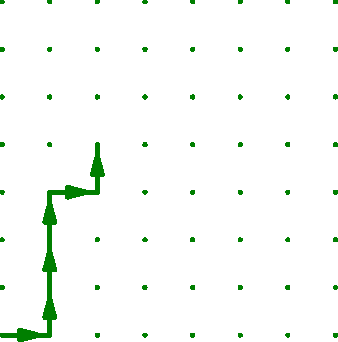
\includegraphics{C2003_4.pdf}
  % C2003_4.pdf: 197x198 px, 72dpi, 6.95x6.99 cm, bb=0 0 197 198
  \caption{Chemin à coordonnées entières.}
  \label{fig:c2003_4}
\end{figure}
On considère le réseau $\N\times \N$ des points à coordonnées entières et les chemins qui partent de l'origine (coordonnées $(0,0)$. Sur un chemin, on passe d'un point au suivant en ajoutant $+1$ soit à l'abscisse soit à l'ordonnée (mais pas aux deux).\newline
Pour $n\in \N$ et $p\in \llbracket 0, n \rrbracket$, on note $c(n,p)$ le nombre de chemins partant de l'origine et se terminant au point de coordonnées $(p,n-p)$.
\begin{prop}
  \begin{displaymath}
    c(n,p) = \binom{n}{p}
  \end{displaymath}
\end{prop}
\begin{figure}[h!]
  \centering
  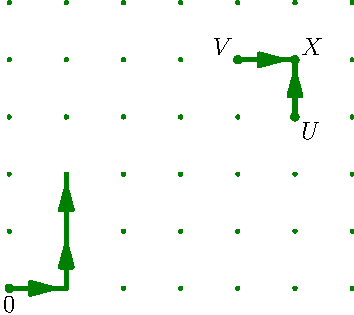
\includegraphics{C2003_5.pdf}
  % C2003_5.pdf: 162x164 px, 72dpi, 5.72x5.79 cm, bb=0 0 162 164
  \caption{Dénombrement de chemins}
  \label{fig:C2003_5}
\end{figure}

\begin{demo}
  Encore une fois, la démonstration consiste à vérifier que les $c(n,p)$ vérifient la relation qui \emph{définit} les coefficients du binôme.\newline
  Considérons $c(n+1,p)$ qui désigne le nombre de chemins d'extrémité $X=(p,n+1-p)$. Le dernier segment du chemin est soit vertical soit horizontal. Introduisons les points $U$ et $V$ respectivement de coordonnées $(p,n-p)$ $(p-1,n-(p-1))$. On peut donc classer les chemins de $O$ à $X$ en deux catégories disjointes suivant qu'ils passent par $U$ (il y en a $c(n,p)$) ou qu'ils passent par $V$ (il y en a $c(n,p-1)$). On en déduit
  \begin{displaymath}
    c(n,p) = c(n-1,p) + c(n,p-1)
  \end{displaymath}
\end{demo}
Un chemin est constitué de segments horizontaux et verticaux. Un chemin de $O$ vers $(p,n-p)$ est complètement caractérisé par le choix des $p$ segments horizontaux parmi les $n$ segments que doit contenir le chemin. Ceci justifie la dénomination $\binom{n}{p} =$\og $p$ parmi $n$\fg.

\section{Identités remarquables à retenir}

\begin{align*}
  &|u+v|^2 = |u|^2 + |v|^2 + 2\Re(u \overline{v}|\\
  &(z-u)(z-\overline{u})  = z^2 - 2\Re(u) z + |u|^2 \\
  &z^2 -2\cos \theta z + 1 = (z-e^{i\theta})(z-e^{-i\theta})\\
  &u^p - v^p = (u-v)(u^{p-1} + u^{p-2}v + \cdots + uv^{p-2} + v^{p-1}) \\
  &u^p - 1 = (u-1)(u^{p-1} + u^{p-2}+\cdots + u +1) \\
  &(u+v)^n = \sum _{k=0}^n \binom{n}{k}u^k v^{n-k}= \sum _{k=0}^n \binom{n}{k}u^{n-k} v^{k}
\end{align*}

\end{document}
